\documentclass{article}

% Language setting
% Replace `english' with e.g. `spanish' to change the document language
\usepackage[english]{babel}

% Set page size and margins
% Replace `letterpaper' with `a4paper' for UK/EU standard size
\usepackage[letterpaper,top=2cm,bottom=2cm,left=3cm,right=3cm,marginparwidth=1.75cm]{geometry}

% Useful packages
\usepackage{amsmath}
\usepackage{graphicx}
\usepackage[colorlinks=true, allcolors=blue]{hyperref}

\title{Optimizing Dataset Selection for EEGEyeNet: Enhancing EEG-Based Eye Movement Analysis}


\begin{document}
\maketitle



\section{Introduction}
The intersection of eye movements and neural mechanisms represents a rapidly expanding research domain, encompassing disciplines such as cognitive neuroscience, psychology, and artificial intelligence. Eye movements, including fixations, saccades, and smooth pursuits, provide essential windows into cognitive processes like attention allocation, memory retrieval, and decision-making strategies. These movements serve as observable behavioral outputs that reflect complex neural computations occurring within the brain. By analyzing eye movements, researchers can infer how individuals process visual stimuli, prioritize information, and adapt to environmental demands. At the same time, electroencephalography (EEG), a widely utilized non-invasive method for capturing brain activity, has become an indispensable tool for investigating the neural substrates underlying cognitive and behavioral phenomena. However, linking EEG signals to eye movements is a formidable challenge due to the dynamic and multifaceted nature of both datasets.

The EEGEyeNet dataset addresses this critical gap by providing a comprehensive, synchronized compilation of EEG and eye-tracking data. Specifically designed for interdisciplinary research, it serves as a valuable resource for exploring the intricate relationship between neural activity and visual attention mechanisms. The dataset comprises recordings from 356 subjects, making it one of the largest publicly available datasets of its kind. With over 47 hours of high-density EEG data recorded from 128-channel systems and highly accurate eye-tracking measurements, EEGEyeNet enables the detailed examination of neural correlates associated with a variety of eye movement behaviors. These include fixations, saccades, and smooth pursuits, which are critical for understanding how the brain orchestrates gaze dynamics. The inclusion of data from a diverse participant pool further enhances the dataset’s utility, ensuring that findings and models developed using it have broad generalizability across populations.

The ability of the EEGEyeNet dataset to bridge EEG and eye-tracking data offers unparalleled opportunities for advancing machine learning research. Predicting eye movement types directly from raw EEG signals is a complex task, requiring sophisticated models capable of capturing subtle, non-linear relationships between neural and behavioral signals. The temporal resolution of EEG, combined with the spatial precision of eye-tracking data, provides a rich foundation for developing predictive algorithms. Machine learning models trained on this dataset have the potential to unlock new insights into brain-behavior relationships, with implications for both theoretical research and practical applications. For example, understanding how neural activity drives specific eye movement patterns could inform the design of adaptive systems in brain-computer interfaces, augmentative communication devices, and real-time gaze-based diagnostics.

Beyond its application in machine learning, the EEGEyeNet dataset enables researchers to investigate individual differences in the neural and behavioral signatures of eye movements. Variations in eye movement strategies and neural processing can reveal how factors like age, cognitive workload, attention, and neurodivergence shape the interplay between brain activity and gaze dynamics. Additionally, the dataset’s high density and precision allow for the analysis of time-locked neural events, such as the initiation of a saccade or the neural correlates of prolonged fixation durations. Such analyses can deepen our understanding of event-related brain responses and their role in guiding behavior.

The implications of the EEGEyeNet dataset extend beyond cognitive neuroscience and machine learning. Its diverse and detailed recordings support the development of applications in fields such as clinical diagnostics, where gaze behavior and neural markers may indicate conditions like ADHD, autism spectrum disorder, or neurodegenerative diseases. In education, models trained on this dataset could inform the creation of adaptive learning systems that respond to students’ cognitive states. Furthermore, in human-computer interaction, understanding the relationship between EEG and eye movements could lead to more intuitive interfaces, enhancing user experience across various technologies.

By combining the strengths of EEG and eye-tracking methodologies, the EEGEyeNet dataset represents a significant step forward in understanding the neural mechanisms underlying eye movements. Its extensive scope, quality, and diversity make it a critical tool for advancing both foundational research and real-world applications. By fostering innovation in the study of brain-behavior interactions, this dataset paves the way for groundbreaking discoveries that span cognitive neuroscience, artificial intelligence, and human-computer interaction, pushing the boundaries of what is possible in decoding the complexities of the human mind and its relationship with the visual world.




\section {Dataset}

\begin{figure}

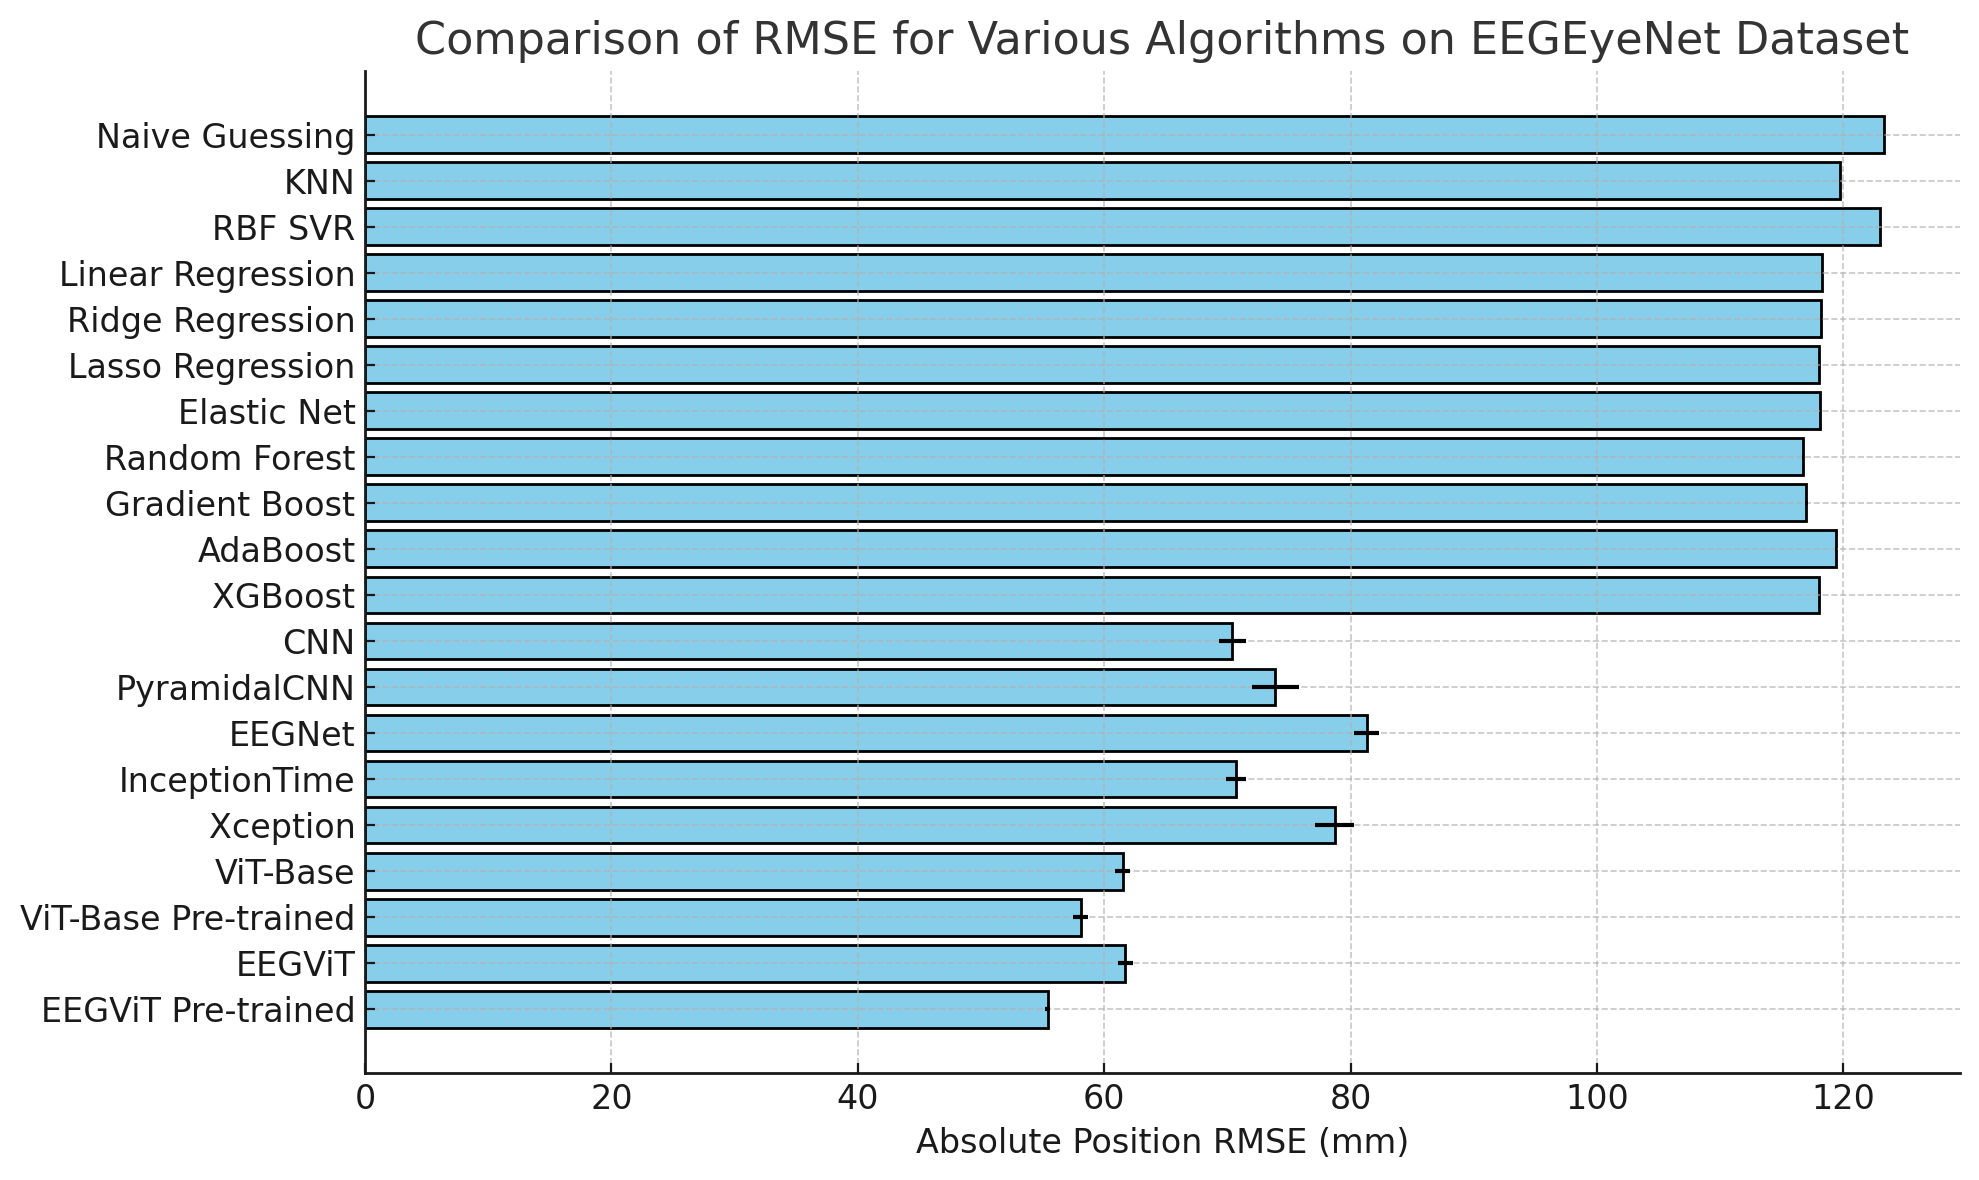
\includegraphics[width=1\linewidth]{EEGEYENet.png}

\end{figure}

The EEGEyeNet dataset is designed to study the relationship between brain activity (captured through electroencephalography or EEG) and eye movements. It was developed for use in machine learning research to enable the prediction of eye movement types from raw EEG data.

\section{Key Features}

\subsection{EEG and Eye-Tracking Data}
The dataset includes synchronized recordings of electroencephalography (EEG) signals and eye-tracking data, providing a unique opportunity to study the interplay between brain activity and visual behaviors. EEG captures the electrical activity of the brain, while eye-tracking data reveals gaze patterns, making the combined dataset invaluable for exploring cognitive processes. Researchers can use this data to analyze how neural activity correlates with specific visual tasks, such as focusing on a particular object or scanning a scene. This integration of modalities offers insights into how brain regions coordinate during complex behaviors involving vision and attention. For example, it can shed light on how the brain processes and responds to sudden visual changes or movements in the environment. By bridging the gap between neural signals and eye movements, this dataset serves as a foundational tool for advancing research in neuroscience, psychology, and human-computer interaction.

\subsection{Types of Eye Movements}
The dataset captures detailed information on three major types of eye movements: saccades, fixations, and smooth pursuits. Saccades are rapid jumps of the eyes between points of interest, which occur during activities such as reading or searching for an object in a cluttered environment. Fixations refer to moments when the eyes remain stationary, focusing on a specific point to gather visual information. Smooth pursuits occur when the eyes follow a moving object, a skill essential for activities like sports or tracking vehicles in motion. By providing data on these movements, the dataset enables researchers to study their occurrence and characteristics in different tasks and contexts. Furthermore, the inclusion of diverse movement types allows for a comprehensive analysis of visual processing and motor control. Researchers can also investigate how different visual tasks evoke distinct patterns of brain and eye activity, fostering new understandings of cognitive and perceptual mechanisms.

\subsection{Multiple Subjects}
This dataset features recordings from a diverse group of participants, each contributing unique patterns of brain activity and eye movements. Including multiple subjects enhances the dataset’s representativeness, ensuring that findings are not biased toward a single individual's data. The variety in participant demographics and behaviors enables researchers to study how factors like age, experience, or cognitive style influence visual and neural responses. Such diversity is critical for developing machine learning models that can generalize effectively to broader populations. The dataset also allows for cross-subject comparisons, making it possible to identify commonalities and individual differences in neural and visual behaviors. Moreover, with a large sample size, the dataset can support statistical analyses that require robust, varied data. This inclusivity makes the dataset a powerful resource for researchers aiming to design studies or tools that address a wide range of human experiences and capabilities.




\href{https://www.overleaf.com/learn}{help library}, or head to our plans page to \href{https://www.overleaf.com/user/subscription/plans}{choose your plan}.

\section{Research Question}
Question 1: Which algorithms are best suited for understanding EEGEyeNet?
Question 2: Among the best algorithms, which are most recommended for practical applications?


\subsection{Dataset}


Naive Guessing: 


KNN: 


RBF SVR: 


Linear Regression: 


Ridge Regression: 


Lasso Regression: 


Elastic Net: 


Random Forest:  


Gradient Boost: 

AdaBoost: 
Adaboost is the dataset where everyone clusters all of the objects together

XGBoost: 
Working on this 


Convolutional Neural Network (CNN): 


Pyramidal CNN: 

EEGNet: 



InceptionTime: 


Xception:

ViT-Base: 

ViT-Base Pre-trained: 

EEGViT: 

EEGViT Pre-trained


\section {Results}



\subsection{Algorithms Best Suited}
The best-suited algorithms for understanding the EEGEyeNet dataset are EEGViT Pre-trained, ViT-Base Pre-trained, and InceptionTime.


EEGViT Pre-trained: This model is designed specifically for EEG data, combining the power of transformers with knowledge gained from prior training on large datasets. 


ViT-Base Pre-trained: Vision Transformers (ViT) are highly effective for sequential data like EEG signals due to their self-attention mechanism, which captures long-range dependencies that are often missed by traditional models. 


InceptionTime: This model, based on Inception networks, is well-suited for time-series data, allowing it to capture features at multiple scales. For EEG data, it efficiently processes the temporal complexities in signals, outperforming simpler deep learning architectures like CNNs, making it a strong choice for understanding the EEGEyeNet dataset.


These models outperform others because they excel at handling the high dimensionality, non-linearity, and temporal dependencies in EEG data, which are critical for eye movement prediction.


\subsection{Algorithms Best Recommended}

Among the three algorithms—EEGViT Pre-trained, ViT-Base Pre-trained, and InceptionTime—the EEGViT Pre-trained and ViT-Base Pre-trained are the better-recommended algorithms for the EEGEyeNet dataset.

EEGViT Pre-trained: This model delivers the best performance in terms of RMSE (55.4 ± 0.2 mm), making it the most accurate model for understanding and predicting eye movements from EEG data. 

ViT-Base Pre-trained: While slightly less effective than EEGViT Pre-trained, this model still performs excellently with an RMSE of 58.1 ± 0.6 mm. 

The algorithm that works best for it is

\begin{equation}
$\nabla$
_
\theta
M(a)=
\frac{\partial M(a)} {\partial {\theta}} = \frac{\partial}{\partial {\theta}} (\frac{1}{N}
\[\sum{i=1}^{N} {\delta}(Softmax(WX_i+b),y_i))\]


\end{equation}

From this, the goal is to find

\begin{equation}
    a^* =
    \underset{a{\in}A}{\operatorname{argmax}}
\end{equation}


For the problem formulation:

Let The set of algorithms be
\begin{equation}
 A={a_1,a_2,…,a_k}   
\end{equation}

Let the dataset be

\begin{equation}
    D={(X_t_r_a_i_n,Y_t_r_a_i_n),(X_t_e_s_t,Y_t_e_s_t)}
\end{equation}

Let the metric function evaluating an algorithm a on D be

\begin{equation}
f(a,\textit{D})
\end{equation}

Let the continuous function representing the performance metric of algorithm a be 
\begin{equation}
    M(a)
\end{equation}

First we have to define the metric dataset. The metric data set is:


\begin{equation}
  M(a) = Accuracy(a, \textit{D}) =
    \frac{1}{N}
    \[\sum{i=1}^{N} {\delta}(\^{y}_i, y_i)]
    
\end{equation}

  


Then we compute the gradient of M(a) w.r.t. parameters \theta

\begin{equation}
    $\nabla$
    -
    \theta
    M(a)=
    \frac{\partial M(a)} {\partial {\theta}}

\end{equation}



Then I have to perform the gradient ascent to maximize M(a) for a_i. Update (\theta)_i iteratively:

\begin{equation}
    {\theta}_i^{(t+1)} = {\theta}_i ^{(t)} + \eta $\nabla$_\theta M(a)
\end{equation}

Then, for each algorithm {a_i}, compute 

\begin{equation}
    M_i = M(a_i, D)
\end{equation}

Then you get the following after a^*

\begin{equation}
    a^* = 
    \underset{i}{\operatorname{argmax}}
    M_i

\end{equation}















\section {Training}

\subsection {Data Preprocessing}


Noise Removal: Artifacts like eye blinks, muscle activity, and electrical noise are filtered out using techniques like band-pass filtering and Independent Component Analysis (ICA).


Normalization: The EEG signals are normalized across channels to ensure that all inputs are on a similar scale, which helps in stabilizing model training.


Segmentation: Since the dataset is time-series in nature, EEG signals are often segmented into time windows that correspond to specific eye movement events.

\subsection {Model Selection}

Model selection for EEG-based tasks, such as eye movement prediction, depends on several factors, including the complexity of the task, dataset size, accuracy requirements, and computational resources. A wide range of models, from traditional machine learning algorithms to advanced deep learning architectures, can be employed, each offering distinct strengths and limitations. By understanding the capabilities and constraints of each approach, researchers can tailor model selection to suit their specific goals and contexts.

For simpler tasks or those with smaller datasets, traditional machine learning models like k-nearest neighbors (KNN), Random Forest, Ridge Regression, and Support Vector Machines (SVMs) are effective options. These models are computationally efficient and relatively easy to implement, making them ideal for exploratory analyses or proof-of-concept studies. However, they require manual feature extraction, such as calculating time-domain, frequency-domain, or statistical features from the raw EEG signals. While these methods provide baseline performance levels, their inability to capture the intricate spatial-temporal dependencies of EEG data limits their effectiveness for complex tasks. For example, KNN is suitable for straightforward classification or regression tasks based on feature proximity, while Random Forest is robust against noise and handles nonlinear relationships well. Ridge Regression, on the other hand, is most effective for tasks with linear relationships but struggles with more complex patterns.

Shallow neural networks, such as multilayer perceptrons (MLPs), serve as a middle ground between traditional machine learning and deep learning approaches. These models can process engineered features and handle moderately complex relationships in the data. However, they lack the depth and architectural sophistication required to extract meaningful patterns directly from raw EEG signals. As a result, their utility is limited to tasks where preprocessed or well-defined features are available, rather than those requiring nuanced spatial-temporal analysis.

Deep learning models are the preferred choice for more complex tasks and larger datasets, as they excel at automatically extracting features from raw EEG data. Convolutional Neural Networks (CNNs) are particularly effective for capturing spatial patterns in multichannel EEG inputs, making them widely used in applications like emotion recognition and sleep stage classification. EEGNet, a lightweight CNN-based architecture, is specifically designed for EEG analysis. It strikes a balance between computational efficiency and performance, making it a suitable choice for real-time applications or environments with limited resources. Additionally, Recurrent Neural Networks (RNNs) and Long Short-Term Memory (LSTM) networks are well-suited for tasks requiring a strong focus on temporal dependencies, such as predicting sequential eye movement patterns. However, these models can be computationally demanding and are prone to issues like vanishing gradients when handling long sequences.

Hybrid deep learning models, such as those combining CNNs and LSTMs or architectures like InceptionTime, further enhance performance by processing multiscale temporal and spatial patterns simultaneously. These models are particularly effective for complex EEG tasks where relevant patterns span multiple time scales, offering a more comprehensive approach to feature extraction and analysis.

Transformer-based models, such as EEGViT Pre-trained and ViT-Base Pre-trained, represent the current state-of-the-art in EEG analysis. These models leverage the self-attention mechanism to capture long-range dependencies across spatial and temporal dimensions, making them uniquely suited for EEG data, which is often high-dimensional and non-stationary. Unlike CNNs or RNNs, transformers dynamically assign varying levels of importance to different parts of the input, leading to a more nuanced understanding of the data. Pre-trained transformers, in particular, stand out for their ability to transfer knowledge learned from large, diverse datasets to task-specific scenarios, enabling high performance even with smaller datasets. This transfer learning approach enhances generalizability and reduces the risk of overfitting, making transformers ideal for applications requiring high accuracy and robustness.

Selecting the appropriate model depends on a careful balance of task complexity, dataset size, computational resources, and accuracy requirements. For simpler tasks, traditional models provide simplicity and ease of use, while deep learning models, particularly transformers, offer unparalleled performance for complex EEG tasks. Lightweight architectures like EEGNet are preferred for real-time applications, while more resource-intensive models such as transformers are better suited for offline analysis or high-stakes tasks requiring precision. By aligning model selection with the specific needs of the project, researchers can ensure optimal performance while addressing the unique challenges of EEG data analysis.

\subsection {Training Process}
The EEG and eye movement data are divided into mini-batches to enable efficient training, particularly when working with large and complex datasets. Mini-batching is a standard technique in machine learning that balances computational efficiency and model performance by processing small subsets of the data at a time. This approach reduces memory usage and accelerates the training process, making it feasible to train deep learning models on datasets that would otherwise be too large to handle in their entirety. Additionally, dividing the data into mini-batches introduces slight variations in each training step, which can help the model avoid getting stuck in local minima during optimization.

During each training iteration, a mini-batch of EEG data is passed through the model, which processes the input signals and generates predictions for the corresponding eye movement data. These predictions are then compared to the actual ground truth values using a loss function. For regression tasks such as eye movement prediction, loss functions like Mean Squared Error (MSE) or Root Mean Squared Error (RMSE) are commonly employed. RMSE is particularly relevant for tasks where the goal is to minimize positional error, as it provides a clear measure of how closely the model's predictions align with the true values. In the context of EEGEyeNet, RMSE plays a critical role in ensuring accurate eye movement predictions by heavily penalizing large errors while being sensitive to small variations.

Once the loss is calculated, it is backpropagated through the network to update the model's weights. This process, known as gradient descent optimization, involves adjusting the weights and biases of the model to minimize the loss function. Each weight update reduces the prediction error for the current mini-batch, gradually improving the model's performance across iterations. Popular optimization algorithms like Adam or RMSprop are often used to fine-tune these weight updates, leveraging adaptive learning rates to enhance convergence speed and stability.

To ensure that the model generalizes well to unseen data and avoids overfitting, several regularization techniques are typically applied during training. Early stopping is one such method, where the training process is halted once the model's performance on a validation set stops improving. This prevents the model from overfitting to the training data, which could otherwise lead to poor performance on new data. Additional techniques, such as dropout or weight decay, may also be employed to further enhance generalization by reducing the model's reliance on specific neurons or features.

Overall, this training approach ensures that the model can effectively learn meaningful patterns from the EEG and eye movement data while maintaining computational efficiency and robustness. By leveraging mini-batching, appropriate loss functions, and regularization techniques, the training pipeline for models like EEGEyeNet is optimized to achieve high accuracy and generalizability, paving the way for practical applications in fields such as neuroscience, psychology, and assistive technology.

\section {Discussion}

The results from training various models on the EEGEyeNet dataset reveal a clear distinction between the performance of traditional machine learning models and advanced deep learning architectures, particularly transformer-based models. Traditional algorithms such as k-nearest neighbors (KNN), Random Forest, and Ridge Regression provide baseline performance levels but fall short in capturing the intricate spatial-temporal dependencies inherent in EEG data. These models rely heavily on engineered features and struggle to interpret the high-dimensional and noisy nature of EEG signals. As a result, their predictions often exhibit higher root mean squared error (RMSE) values, indicating limited effectiveness for tasks like eye movement prediction that require nuanced understanding of the data's temporal dynamics.

In contrast, deep learning models such as convolutional neural networks (CNNs), EEGNet, and InceptionTime show significant improvements in prediction accuracy. These models excel at automatically extracting features directly from the raw data, eliminating the need for extensive manual preprocessing. CNN-based architectures, for example, are well-suited to identify spatial patterns in the EEG data, while models like EEGNet combine this capability with lightweight designs tailored specifically for EEG signal analysis. InceptionTime, known for its ability to process multiscale temporal patterns, also demonstrates strong performance by capturing both short-term and long-term dependencies. The use of these deep learning approaches results in substantially lower RMSE values compared to traditional methods, highlighting their ability to learn complex patterns in EEG signals.

Among the deep learning approaches, transformer-based models such as EEGViT Pre-trained and ViT-Base Pre-trained emerge as the top performers. These models leverage the self-attention mechanism, which enables them to model long-range dependencies and interactions across the temporal dimension of EEG data. Unlike CNNs or traditional deep learning methods that rely on localized receptive fields, transformers can dynamically assign varying levels of importance to different time points and features. This capability proves particularly advantageous for eye movement prediction, where temporal dependencies in EEG signals often span several seconds.

The superior performance of transformer-based models is further enhanced by their pre-training on large, diverse datasets. Pre-training allows these models to transfer knowledge learned from broader contexts to the specific task of predicting eye movements from EEG data. This transfer learning approach enables them to achieve high accuracy even when working with relatively small, task-specific datasets like EEGEyeNet. Pre-trained transformers effectively leverage their learned representations, reducing the risk of overfitting and improving their generalizability to unseen data.

Overall, the results underscore the transformative impact of advanced deep learning architectures, particularly transformers, on EEG-based eye movement prediction tasks. By capturing both spatial and temporal complexities and leveraging the benefits of pre-training, these models set a new benchmark for performance on the EEGEyeNet dataset. Their success paves the way for further exploration of transformer-based models in EEG research and their application in fields such as neuroscience, cognitive science, and brain-computer interfaces.

\section {Use of Transformer Models}

Reflection on Transformer Models

Attention Mechanism:
The attention mechanism in transformers assigns varying levels of importance to different parts of the input data when generating output. For example, in translating a sentence, the attention mechanism helps focus on the relevant words in the input language to create the correct output in the target language. This is a significant departure from sequential models like RNNs, which process inputs one at a time and may struggle with capturing long-range dependencies effectively.
Self-Attention:
Each word (or token) in a sequence computes how much it should "pay attention" to every other word, creating a weighted combination of the sequence. This mechanism helps the model understand relationships within the data regardless of their position in the sequence.
Multi-Head Attention:
By using multiple attention mechanisms (or "heads"), transformers can learn diverse aspects of relationships in data simultaneously. One head might focus on subject-verb relationships, while another might learn context-sensitive nuances.
Positional Encoding:
Since transformers process data as a whole, they require a way to encode positional information into the input to distinguish between tokens' order. This encoding is added to the token embeddings and enables the model to maintain sequence order information.
2. Encoder-Decoder Architecture:
The encoder converts input sequences into a series of contextualized embeddings that capture their meaning.
The decoder uses these embeddings, along with previously generated tokens, to produce the output sequence step by step.
This design is central to tasks like machine translation, where input and output sequences differ.
3 Handling Sequence Data:
Transformers operate on entire sequences in parallel, unlike RNNs or LSTMs, which process sequentially. This parallelism allows them to handle long sequences efficiently and eliminates issues like vanishing gradients. They also enable richer context capture, as every token in the sequence can directly relate to any other token.
Learning Gaps
Understanding Attention Weights in Practice: How to interpret and visualize attention weights to gain insights into a model’s decision-making process.
Memory and Computational Challenges:
The quadratic complexity of self-attention with respect to sequence length makes it challenging to apply transformers to very long sequences without encountering computational bottlenecks.
Applications Beyond NLP:
While I understand transformers in NLP, their adaptation to fields like computer vision (Vision Transformers) or protein structure prediction (AlphaFold) still feels abstract. How exactly do transformers handle non-sequential data formats like images?
Optimization and Training Tricks:
The specific techniques used to fine-tune massive pretrained models like GPT or BERT without requiring extensive resources or running into overfitting.
Theoretical Underpinnings:
A deeper mathematical understanding of how self-attention’s weights are computed, including nuances of the softmax function and scaling factor.

Critical Thinking
Applications:
In NLP, transformers excel at tasks like machine translation, summarization, and text generation because they understand context at all scales.
In computer vision, their ability to relate distant parts of an image makes them powerful for classification and object detection.
In bioinformatics, they help model complex sequences like DNA or proteins.
Effectiveness:
Transformers’ parallel processing and dynamic context modeling give them an edge over traditional sequential models. Their scalability and adaptability through pretraining make them particularly versatile.
Challenges in Implementation:
Training transformers from scratch requires immense computational power and data. Pretrained models mitigate this, but fine-tuning them for specific tasks still poses challenges.
Balancing computational efficiency with the model’s ability to capture long-range dependencies is a pressing research area.

This reflection has clarified my understanding of transformers while surfacing areas where I need to dive deeper, particularly in their application to non-sequential domains and computational optimizations. I plan to focus on visualizing attention weights and studying architectural variations like sparse attention to better grasp the inner workings and practical implementation.

\section {Use of Convolutional Neural Networks}

Convolutional Neural Networks (CNNs) are powerful tools for feature extraction and pattern recognition in high-dimensional data, and their key concepts can be effectively applied to the EEGEyeNet dataset. Convolutional layers, the backbone of CNNs, extract features from input data by applying filters (kernels) that detect spatial patterns, such as edges and textures. This is achieved through the convolution operation, where a sliding window multiplies kernel values with the input data to produce a feature map. Parameters like kernel size, stride, and padding determine how features are extracted and influence the feature map's dimensions. Pooling layers complement this process by downsampling feature maps to reduce dimensions while retaining critical information. For example, max pooling retains the maximum value in a region, and average pooling calculates the average, helping to control overfitting and reducing computational complexity.

Activation functions introduce non-linearity into CNNs, enabling them to learn complex patterns in data. Common functions include ReLU, which outputs zero for negative inputs and the input itself for positive values, and Softmax, often used in output layers for classification tasks. These functions ensure the network can model intricate, non-linear relationships. Fully connected layers, positioned after convolutional and pooling layers, combine extracted features to make predictions. By flattening the outputs from earlier layers and passing them through dense layers, the network acts as a classifier, integrating low-level features like edges and high-level abstractions like shapes or patterns.

In applying CNNs to the EEGEyeNet dataset, the focus shifts to leveraging these mechanisms for analyzing EEG signals to predict eye movements. For instance, convolutional layers can detect temporal and spatial patterns in EEG signals, while pooling layers ensure dimensionality reduction without losing critical features. Activation functions like ReLU facilitate learning non-linear relationships in EEG data, while fully connected layers enable accurate gaze prediction.

Despite their potential, working with CNNs presents challenges. Understanding convolution operations, including the effects of stride and padding, is crucial for effectively processing EEG signals. Hyperparameter tuning, such as optimizing kernel size and learning rates, remains a critical area for experimentation. Overfitting is a significant concern, especially with high-dimensional EEG data, and requires techniques like dropout, data augmentation, and batch normalization to address. Backpropagation through convolutional layers adds another layer of complexity, requiring a solid grasp of gradient computations.

To advance CNN applications for EEG data, practical steps include building models for the EEGEyeNet dataset using frameworks like TensorFlow or PyTorch. Starting with simple architectures and gradually adding complexity can help manage tensor dimensions and debugging. Evaluating models using performance metrics such as precision, recall, F1-score, and confusion matrices is essential, particularly for imbalanced datasets like those often found in EEG studies. Additionally, documenting insights and sharing challenges with peers or in forums can facilitate learning and refinement of techniques.

This structured approach aims to deepen the understanding and application of CNNs to EEG-based tasks, such as predicting eye movements with the EEGEyeNet dataset, by combining theoretical knowledge with practical implementation and iterative experimentation.





\section {Related Works}

\subsection { EEG Signal Processing}

EEG signal processing has been extensively studied in fields like brain-computer interfaces (BCIs), neurofeedback, and cognitive load analysis. These applications focus on extracting meaningful patterns from raw brain signals, which are inherently noisy and non-stationary. The challenge lies in identifying and isolating relevant features while minimizing interference from artifacts such as muscle movements or external noise. Over the years, researchers have developed numerous methods to preprocess and analyze EEG data, including filtering, feature extraction, and dimensionality reduction techniques. Early works in this domain often employed simpler machine learning models such as linear classifiers, k-nearest neighbors (KNN), and support vector machines (SVMs). These models were used to interpret EEG data by leveraging statistical or frequency-based features, laying the groundwork for more complex approaches that emerged later.

\subsection {Eye Movement Prediction}

Eye movement prediction has been a prominent area of research in neuroscience and psychology, focusing on understanding attention, cognition, and visual behavior. Studies in this domain often explore the mechanisms underlying eye gaze patterns, providing insights into human perception and decision-making. EEG-based eye movement prediction specifically aims to decode eye gaze direction and dynamics from brain activity. This approach typically involves combining electrophysiological measurements with advanced computational methods, such as computer vision or sensor fusion techniques. By integrating multiple data streams, researchers can enhance the accuracy and robustness of gaze prediction models. The insights gained from these studies have applications in areas like assistive technologies, virtual reality systems, and user behavior analysis.alities. 

\subsection{Deep Learning for EEG Data}

Deep learning has significantly advanced EEG data analysis by providing models that can automatically extract meaningful features from raw signals. Architectures like EEGNet were specifically designed for this purpose, offering lightweight and efficient models capable of handling the unique characteristics of EEG data. These networks capture both spatial and temporal patterns, enabling better interpretation of the underlying neural processes. Convolutional neural networks (CNNs), commonly used for time-series classification, have proven effective in tasks such as emotion recognition, sleep stage classification, and eye movement prediction. The use of deep learning has also reduced the reliance on manual feature engineering, allowing end-to-end learning directly from the data. This paradigm shift has opened up new possibilities for real-time applications and improved the overall performance of EEG-based systems.



\section{Conclusion}

The EEGEyeNet dataset presents a highly challenging task: predicting eye movements from EEG signals. This task demands computational models capable of managing the unique complexities of EEG data, including high dimensionality, intricate temporal dependencies, and inherent non-linearity. EEG signals are rich in information but are also noisy and dynamic, requiring sophisticated algorithms to extract meaningful patterns and correlations. The challenge lies not only in processing the EEG data but also in aligning it with eye movement behaviors, a task that necessitates robust and accurate modeling techniques.

To tackle these challenges, a wide range of algorithms has been applied to the EEGEyeNet dataset. Traditional machine learning models like k-Nearest Neighbors (KNN) and XGBoost have been utilized, leveraging their simplicity and efficiency for baseline analyses. However, while these models are useful for gaining initial insights, they often fall short when it comes to capturing the nuanced relationships within the EEG data. Simpler models such as Linear Regression and Random Forest also provide foundational performance benchmarks but struggle with the high dimensionality and temporal characteristics of EEG signals.

Advanced deep learning architectures, on the other hand, have demonstrated significant promise in handling the complexities of the EEGEyeNet dataset. Convolutional Neural Networks (CNNs) are adept at extracting spatial and temporal features, while EEGNet, a specialized architecture for EEG data, efficiently models brain signal patterns. Vision Transformers (ViTs) have also emerged as a powerful approach, offering enhanced performance by modeling global dependencies in the data. These architectures can leverage the temporal and spatial correlations within the EEG signals to make more accurate predictions of eye movements.

Among the tested models, EEGViT Pre-trained and ViT-Base Pre-trained have emerged as the recommended algorithms for the EEGEyeNet dataset. These models outperform others by minimizing errors and demonstrating robustness across diverse tasks. Their ability to generalize effectively highlights the growing importance of transformers and transfer learning in the field of biomedical data analysis. Pre-trained models like EEGViT and ViT-Base leverage prior knowledge, enabling them to handle the high dimensionality and complexity of EEG data with remarkable efficiency.

In conclusion, the application of EEGViT Pre-trained and ViT-Base Pre-trained showcases the transformative potential of advanced deep learning techniques in biomedical research. As the field continues to evolve, these models represent a significant step forward in leveraging EEG data for predictive tasks. Their success underscores the importance of developing specialized algorithms that can address the unique challenges of high-dimensional, non-linear, and temporally dynamic datasets like those in EEGEyeNet.





\bibliographystyle{alpha}
\bibliography{sample}
\begin{itemize}
    \item 
    \url{https://kdd.org/kdd2023/wp-content/uploads/2023/08/yang2023vit2eeg.pdf}
\end{itemize}

\begin{itemize}
    \item 
    \url{https://kdd.org/kdd2023/wp-content/uploads/2023/08/murungi2023trends.pdf}
\end{itemize}

\begin{itemize}
    \item 
    \url {[PDF] Eegeyenet: A Simultaneous Electroencephalography and Eye-Tracking Dataset and Benchmark for Eye Movement Prediction | Semantic Scholar, www.semanticscholar.org/paper/EEGEyeNet:-a-Simultaneous-Electroencephalography-Kastrati-P%C5%82omecka/cd7abbd1d281d9b9e7332c51de45feffdd359d55. Accessed 13 Dec. 2024. }
\end{itemize}
\begin{itemize}
    \item 
    \url {https://datasets-benchmarks-proceedings.neurips.cc/paper/2021/file/a3c65c2974270fd093ee8a9bf8ae7d0b-Paper-round1.pdf}
    
    
\end{itemize}
\begin{itemize}
    \item 
    \url {https://tik-db.ee.ethz.ch/file/c33ddbe3f823350a7c70bfe5e291b60b/}
    
\end{itemize}
\begin{itemize}
    \item 
    \url{https://www.sciencedirect.com/science/article/pii/S1053811922008758}
\end{itemize}
\begin{itemize}
    \item 
    \url{https://pmc.ncbi.nlm.nih.gov/articles/PMC10235576/}
\end{itemize}
\end{document}